\section{Pulsdetektering}\label{sec_de_im_te_puls}
\textit{Dette afsnit beskriver design, implementering og test af pulssensoren og den tilhørende algoritmen. Pulssensoren er en færdigudviklet komponent, hvorfor afsnittet er særligt omhandlende algoritmen til pulsdetektering. Først designes opsætningen af pulssensoren og dets algoritme til det specifikke formål, hvorefter dette implementeres. Afslutningsvist bliver algoritmen vedrørende pulsdetektering testet i forhold til opstillede krav i \secref{puls_krav}.}

\subsection{Design} \label{sec_design_puls}
Pulssensoren skal benyttes til at beskrive intensiteten af aktiviteten, som er beskrevet i \secref{subsub:ak_int}. Heraf kan effekten af aktiviteten bestemmes, hvilket vil blive benyttet som en motiverende faktor i forbindelse med visualisering i GUI. \newline
Pulssensoren SEN-11574 er valgt til dette projekt, da den er en optisk pulssensor og er derfor særdeles alsidig med henhold til placering, som beskrevet i \secref{sec:pulssensor}. En optisk sensor påkræver blot en placering over en arterie for at kunne måle pulsen, som følge af blodets gennemstrømning. Eksempelvis kan den optiske sensor placeres på fingerspidsen eller øreflippen, hvoraf denne rapport benytter øreflippen. Dette skyldtes, at ved en placering på øreflippen er der mindre bevægelse af sensor og ledninger end ved en fingerspids, hvormed mængden af støj kan reduceres. \\
SEN-11574 kræver en spændingstilkobling på 3~V til 5~V for at være funktionel og forbruger 4~mA ved en forsyning på 5~V. På sensorens printplade findes et aktivt filter\fxnote{Et aktivt filter er en type af analog elektronisk filter, der anvender aktive bestanddele, såsom en forstærker.} samt en forstærker, som tilsammen øger amplituden for pulsbølgen og normaliserer signalet omkring et referencepunkt, hvilket fjerner DC spænding i signalet. \citep{Murphy2016,Murphy2016_sensor}\\
Pulssensoren designes således, at pulsen (BPM) beregnes for brugeren i GAP peripheral og sendes til GAP central, hvilket fremgår af \figref{fig:puls_pseudo}.
\begin{figure}[H]
	\centering
	\includegraphics[scale=0.6]{figures/cDesign/puls_pseudo.png}
	\caption{På figuren ses et flowchart over algoritmen vedrørende detektering af BPM. Pulssensorens algoritme skal registrere fem pulsslag som overskrider en given tærskelværdi, førend BPM kan bestemmes med udgangspunkt i disse værdier.}
	\label{fig:puls_pseudo}
\end{figure}
Ovenstående figur repræsenterer algoritmen vedrørende detektering af BPM. Pulssensoren opfanger pulssignalet fra brugerens øreflip, hvorefter dette signal bliver signalbehandlet førend detektering af pulsslag startes. Der ønskes at detektere pulsen ved at beregne varigheden mellem tre pulsslag med udgangspunkt i det systoliske peak, hvilket fremgår af \secref{sec:pulssensor}. Dette peak har større amplitude end peaket for diastole, hvormed signalbehandlingen skal forstærke det systoliske peak og dæmpe det diastoliske peak.  \\
Dataet fra pulssensoreren signalbehandles i form af en division og kvadrering. Dette vil medføre, at det største peak i signalet vil blive forøget i amplitude, og de mindre peaks vil opnå en lavere amplitude, hvilket ses på \figref{fig:behandlet_puls}. 
\begin{figure}[H]
	\centering
	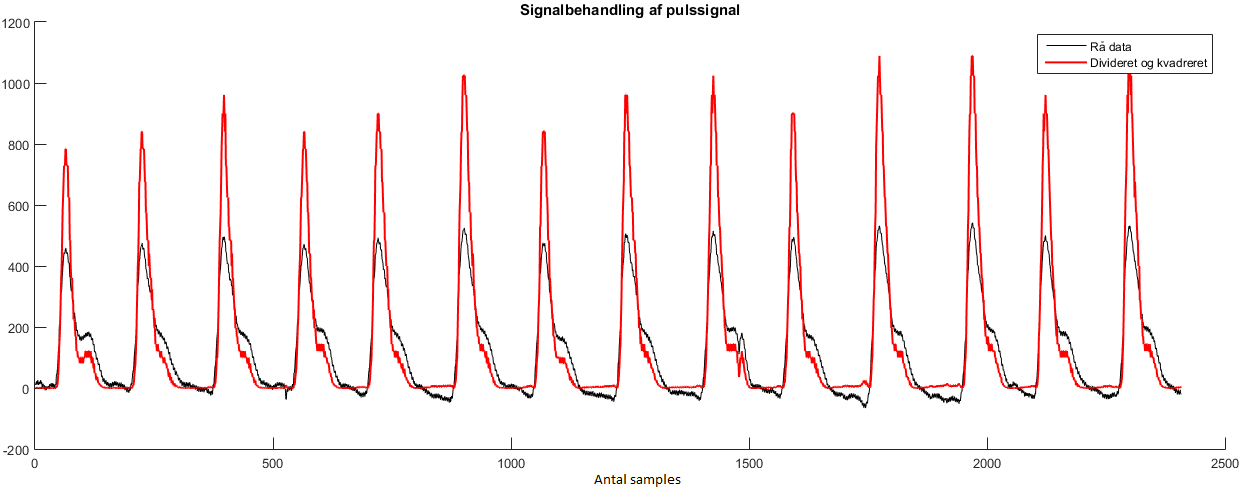
\includegraphics[scale=0.4]{figures/cDesign/puls_ore_behandlet.png}
	\caption{På figuren ses algoritmens signalbehandling af et råt pulssignal. Den sorte kurve er det rå pulssignal, og den røde kurve er det dividerede og kvadrerede signal.}
	\label{fig:behandlet_puls}
\end{figure}
Som resultat af signalbehandlingen på \figref{fig:behandlet_puls} ses det, at amplituden på det behandlede signal er forøget, hvorimod de mindre peaks er formindsket. De største peaks i signalet repræsenterer den systoliske periode i hjertecyklussen, hvilket er det peak, der benyttes til at bestemmes BPM for signalet. For at kunne bestemme BPM for signalet, bliver der implementeret en tærskelværdi. Denne værdi skal signalet overskride for at kunne blive detekteret som et systolisk peak. Tærskelværdien for algoritmen bestemmes med udgangspunkt i en pulsmåling, hvor sensoren er placeret på øreflippen. Dette fremgår af \figref{fig:taerskel_puls}.
\begin{figure}[H]
	\centering
	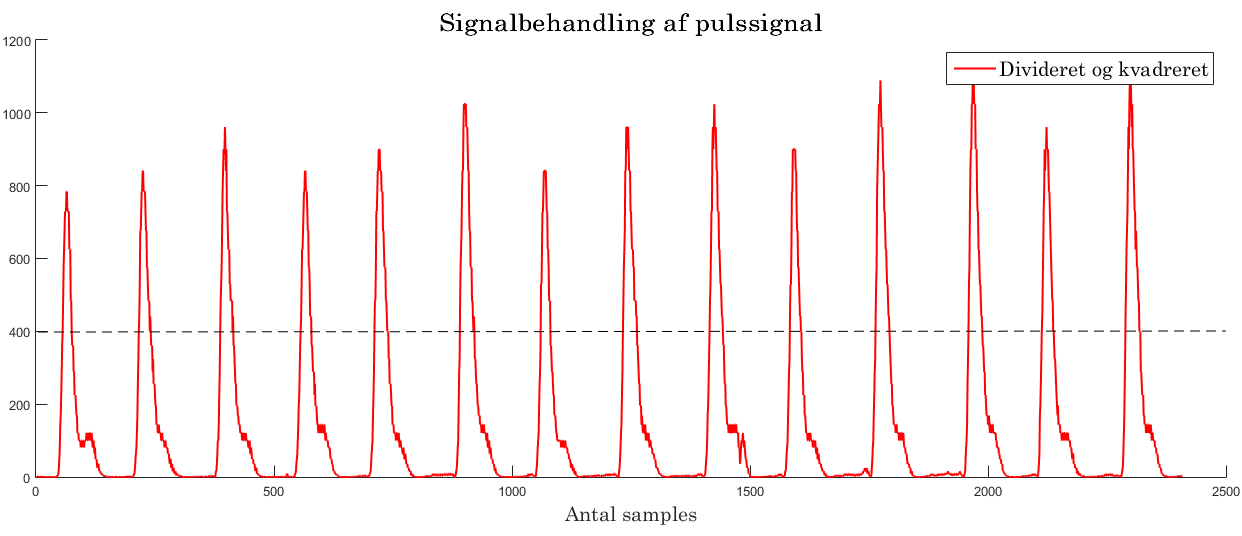
\includegraphics[scale=0.4]{figures/cDesign/puls_taerskel.png}
	\caption{På figuren ses en pulsmåling foretaget på øreflippen. Den røde kurve er en signalbehandlet pulsmåling fra øreflippen, og den sorte stiplede linje er algoritmens tærskelværdi, som har en værdi på 400.}
	\label{fig:taerskel_puls}
\end{figure} \vspace{-0.5cm}
Det behandlede signal fremgår af figuren, hvortil der er indtegnet en tærskelværdi på 400, som alle de systoliske peaks vil overskride. Tærskelværdi på 400 vil medføre, at det systoliske tryk overstiger tærskelværdien, hvortil det diastoliste tryk vil befinde sig under. Algoritmen vil benytte varigheden mellem de forekomne systoliske tryk til at kunne beregne BPM med udgangspunkt i fem detekterede peaks. 

\subsection{Implementering} \label{puls_impl}
Pulssensoren har 3 pins til henholdsvis spændingsforsyning, ground og outputsignal. Disse pins kobles til hver sin pin på GAP peripheral. Outputsignalets pin skal designes i PSoC Creator, således MCUen modtager pulssensorens signaler fra den pågældende pin. Dette gøres ved at indsætte henholdsvis en UART serie kommunikationsblok (SCB) og SAR ADC i topdesignet. UARTen bruges til, at sensoren og MCUen kan kommunikere med hinanden. Standardindstillingerne for denne blok benyttes til konfigurationen af MCUen. \newline
Outputsignalet fra sensoren er et analogt signal, hvormed dette signal opsamles af en ADC for at skabe en konvertering til et digitalt signal. ADCens design skal derfor konfigureres således, at denne bearbejder én single ended kanalinput fra pulssensoren. Yderligere indstilles samplingsfrekvensen for ADCen for den pågældende inputkanal til 35~Hz, med henhold til \secref{krav_adc}. \\
Efter konfigurering af UART og ADC i topdesignet, skal de korrekte pins indstilles i pinopsætning. UART tildeles interne RX-, og TX-pins, hvorimod ADCens inputpin skal indstilles til den pin, som outputtet fra sensoren er placeret i, hvilket er valgt til pin 2.0. \\
Med udgangspunkt i de implementerede elementer, bliver der implementeret en algoritme til pulsdetekteringen, som det ses på \figref{fig:puls_pseudo_c}.
\begin{figure}[H]
	\centering
	\includegraphics[scale=0.5]{figures/cDesign/Puls_ckode.png}
	\caption{På figuren ses pulssensorens algoritme i C kode beskrevet med pseudokode. Efter nulstilling af de benyttede variabler, bliver time counteren startet igen, hvorefter løkken fortsætter sin virken.}
	\label{fig:puls_pseudo_c}
\end{figure} \vspace{-0.5cm}
Første trin, efter dataopsamlingen fra pulssensoren, er en konvertering af det analoge signal til et digitalt. Derefter undersøges det, hvorvidt det konverterede data er klar, hvilket der benyttes en indbygget kodegenerering til og beskrives yderligere i \secref{adc_design_impl}. Hvis data er klar, da starter algoritmens time counter som starter optælling af samples. Når en sample er klar, bliver den kvadreret og divideret, som det beskrives i \secref{sec_design_puls}. Den behandlede sample gemmes i en variabel, 'Value[0]'. Når der kommer en ny sample, vil den forrige sample blive gemt i en ny variabel, 'Value[1]', og den nye sample gemmes i den anden variabel. \\
Yderligere tæller algoritmen antallet af pulsslag, ved at vurdere om 'Value[0]' er under tærkselværdien og 'Value[1]' er over. Hvis dette er tilfældet, vil der blive lagt én til antal pulsslag, dog maksimalt til antal pulsslag er <6. Algoritmen er bestemt til at nulstille sin time counter hver gang der registreres tre tilfælde, hvor en sample er gået under tærskelværdien på 400. Derfor vil algoritmen kunne beregne BPM for brugeren, med det forbehold, at antallet af pulsslag skal være fem. Time counteren benyttes i denne forbindelse, til at optælle antallet af samples for fem pulsslag. Beregningen foretages ved at bestemme den gennemsnitlige varighed mellem hvert pulsslag med udgangspunkt i fem pulsslag. Derefter divideres denne varighed med 60 sekunder, for at kunne bestemme BPM. Når beregningen er foretaget, vil BPM for brugeren blive sendt til GAP central gennem BLE, hvorefter algoritmens værdier nulstilles.\\
Efter nulstilling af de benyttede variabler, bliver time counteren startet igen, hvorefter løkken fortsætter sin virken.


\subsection{Test}
Pulssensoren testes, for at undersøge hvorvidt den designede og implementerede algoritme kan bestemme den rigtige puls ved et simuleret signal. Ydermere testes sensoren og algoritmen, ved at benytte Verniers Excercise Heart Rate Monitor, som reference for den puls i BPM som pulssensoren og den tilhørende algoritme bør sende via BLE. \\
Testen udføres på baggrund af
de opstillede krav og tilhørende tilladte afvigelser opstillet i \secref{puls_krav}. Kravene til pulsedetektering, beskriver at pulsdetekteringen skal:
\begin{itemize}
	\item Kunne detektere brugerens puls ved fysisk aktivitet. Der accepteres en afvigelse af pulsen på 10\%.
\end{itemize}

Algoritmens funktionalitet testes ved at indsende et simuleret signal, som består af et absolut sinussignal. Peaks på det simulerede signal skal repræsentere de systoliske peaks i et pulssignal optaget med en pulssensor.\\
Det simulerede signal sendes ind i MCUen, hvorefter det undersøges hvorvidt time counteren detekterer varigheden mellem overskridelser af algoritmens tærskelværdi på 400. Når pulsen er bestemt, benyttes programmet Real Term til at printe algoritmens slutresultat, som er pulsen i BPM. \\
Det indsendte signal har en frekvens på 0,6~Hz og en signals samplingsfrekvens på 35~Hz, samt en længde på 992 samples. Derfor kan det bestemmes hvilken puls, som algoritmen bør printe i Real Term. \\
Der indsendes 992 samples og benyttes en samplingsfrekvens på 35~Hz, hvormed arrayet har en længde på 28,3 sekunder. Idet der er tale om et absolut sinussignal på 0,6~Hz, vil der opstå 34 peaks i det indsendte signal. Dette vil betyde, at algoritmen skal udregne og printe seks værdier for pulsen, idet der er 34 fuldstændige peaks. \\
Når der er 34 peaks og arrayet har en varighed af 28,3 sekunder, vil der være 0,83 sekunder mellem hver overskridelse af tærskelværdien, hvormed pulsen bestemmes, som det fremgår af \eqref{eq:puls_teori}:
\begin{equation}
\frac{60~sekunder}{Varighed~mellem~samples} = \frac{60~sekunder}{0,83~sekunder} = 72~BPM
\label{eq:puls_teori}
\end{equation} 
Derfor vil det indsendte signal medføre en værdi af 72 BPM, hvorfor det er forventeligt, at algoritmen vil beregne og printe en puls, som har en værdi af 72 BPM.

Algoritmen er bestemt til at nulstille time counteren hver gang der registreres fem tilfælde, hvor en sample er gået under tærskelværdien. Derfor vil algoritmen gøre brug af time counterens optalte antal samples til at bestemme pulsen for den pågældende periode. \\
Ved at indsende det simulerede signal fremgår det af \figref{fig:timecounter_puls_realterm}, hvordan time counteren nulstilles, når der er registreret fem tilfælde. Ydermere ses det i \figref{fig:test_puls_realterm}, at Real Term har printet de forventede værdier for BPM.
\begin{figure}[H]
	\centering
	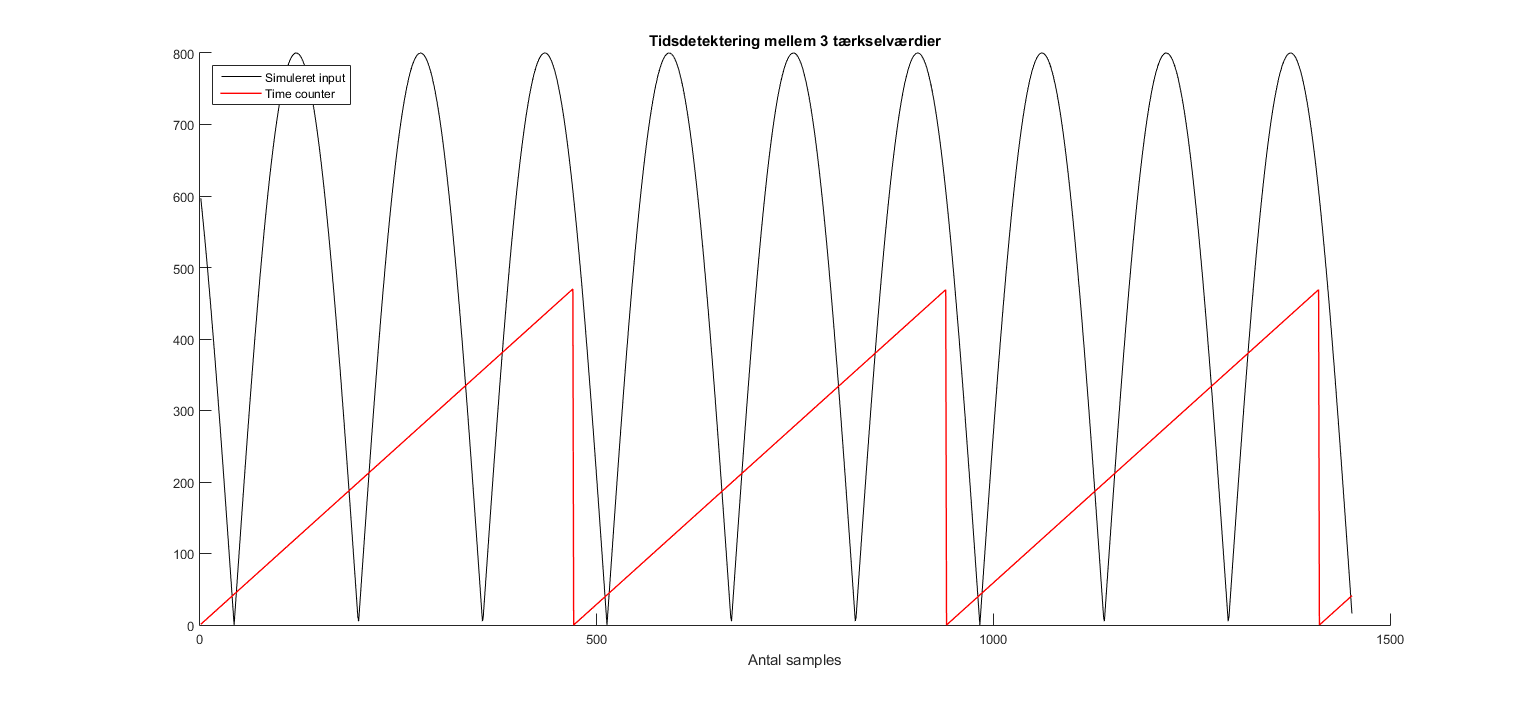
\includegraphics[scale=0.4]{figures/cDesign/timecounter_puls_pic.png}
	\caption{På figuren ses algoritmens time counter, som tæller op, indtil en sample på det femte pulsslag er gået under tærskelværdien. Efterfulgt af dette vil time counteren nulstilles og genstarte optælling af samples.}
	\label{fig:timecounter_puls_realterm}
\end{figure}

Det fremgår af \figref{fig:timecounter_puls_realterm}, at algoritmen tæller indtil fem peaks er detekteret. Herefter beregner algoritmen pulsen ud fra det antal samples, som findes inden for disse fem peaksdetekteringer. Herefter printes pulsen i Realterm, som det fremgår af \tabref{tab:test_puls_realterm}.
\begin{table}[H]
	\centering
	\begin{tabular}{ccc}
		\hline
		\rowcolor[HTML]{C0C0C0} 
		Forventet værdi [BPM] & Modtaget værdi [BPM] & Afvigelse [\%]\\ \hline
		72 - 72 - 72 - 72 - 72 - 72         & 72 - 72 - 72 - 72 - 72 - 72         & 0 - 0 - 0 - 0 - 0 - 0 \\ \hline
	\end{tabular}
	\caption{I tabellen ses resultaterne fra algoritmens beregning af pulsen på et simuleret inputsignal. Tabellens kolonne; Modtaget værdi, er værdierne printet i Real Term.}
	\label{tab:test_puls_realterm}
\end{table} \vspace{-0.5cm}
Det fremgår, at den forventede puls var 72 BPM samt at Real Term modtager og printer en tilsvarende værdi. Det kan derfor konkluders, at algoritmen har 0\% afvigelse på et simuleret inputsignal. \\
Det kan derfor konkluderes, at pulssensoren og den tilhørende algoritme fungerer som tiltænkt ved benyttelse af et simuleret inputsignal. 

Der foretages yderligere tre tests, med henblik på at vurdere hvorvidt pulssensoren opfylder de opstillede krav. Den ene test er ved en stillesiddende position, mens den anden og tredje test er ved fysisk aktivitet i form af henholdsvis gang og løb. Det er gældende for alle tests, at der bliver benyttet en pulsmåler i form af Vernier Excercise Heart Rate Monitor, der benyttes som reference for den beregnede puls af algoritmen. Denne pulssensors data vil blive printet i programmet LoggerPro, og den algoritmebestemte puls vil blive printet i Realterm. \\
Pulssensoren og den tilhørende algoritme testes på en person ved en stillesiddende aktivitet, hvoraf personens puls er forholdsvis stabil og uden markante udsving. Testen udføres ved at have pulssensor påført øreflippen, hvoraf MCUen bestemmer puls i BPM og printer denne værdi i Real Term. \\
Resultaterne af den første udførte test, ved en stillesiddende position, fremgår af \tabref{tab:test_pulssystem}.
\begin{table}[H]
	\centering
\begin{tabular}{ccc}
	\hline
	\cellcolor[HTML]{C0C0C0}\begin{tabular}[c]{@{}c@{}}Gennemsnitspuls \\ LoggerPro {[}BPM{]}\end{tabular} & \cellcolor[HTML]{C0C0C0}\begin{tabular}[c]{@{}c@{}}Gennemsnitspuls \\ algoritme {[}BPM{]}\end{tabular} & \cellcolor[HTML]{C0C0C0}\begin{tabular}[c]{@{}c@{}}Afvigelse \\ {[}\%{]}\end{tabular} \\ \hline
	60 & 64,9 & 8,15 \\ \hline
\end{tabular}
	\caption{I tabellen ses det den gennemsnitlige puls fra LoggerPro og Real Term målt på stillesiddende person. Det fremgår, at pulssensoren og den tilhørende algoritme har en afvigelse på 8,15\%.}
	\label{tab:test_pulssystem}
\end{table} \vspace{-0.5cm}
Det fremgår i \tabref{tab:test_pulssystem}, at testen af pulssensoren og den tilhørende algoritme viser en gennemsnitlig afvigelse fra referenceværdien på 8,15\%. Pulssensoren og den tilhørende algoritme overholder dermed første krav til pulsdetekteringen, ved stillesiddende position.

Anden test undersøger hvorvidt det er muligt at detektere puls under fysisk aktivitet. Denne test indebærer en pulsmåling under fysisk aktivitet i form af gang ved 4,8~km/t på et løbebånd.\\
Resultaterne af den anden udførte test med gang, fremgår af \tabref{tab:test_puls_aktivitet}.
\begin{table}[H]
	\centering
	\begin{tabular}{ccc}
		\hline
		\cellcolor[HTML]{C0C0C0}\begin{tabular}[c]{@{}c@{}}Gennemsnitspuls \\ LoggerPro {[}BPM{]}\end{tabular} & \cellcolor[HTML]{C0C0C0}\begin{tabular}[c]{@{}c@{}}Gennemsnitspuls \\ algoritme {[}BPM{]}\end{tabular} & \cellcolor[HTML]{C0C0C0}\begin{tabular}[c]{@{}c@{}}Afvigelse \\ {[}\%{]}\end{tabular} \\ \hline
		116,5 & 95,70 & 17,85 \\ \hline
	\end{tabular}
	\caption{I tabellen ses det den gennemsnitlige puls fra LoggerPro og Real Term ved gang. Det fremgår, at pulssensoren og den tilhørende algoritme har en afvigelse på -17,85\%.}
	\label{tab:test_puls_aktivitet}
\end{table} \vspace{-0.5cm}
Det fremgår i \tabref{tab:test_puls_aktivitet}, at testen af pulssensoren og den tilhørende algoritme ved 4,8~km/t viser en gennemsnitlig afvigelse fra referenceværdien på -17,85\%. Pulsdetekteringen ved gang overholder derfor ikke det opstillede krav for pulsdetektering.\\
Yderligere testes pulsdetektering ved løb med 11,3~km/t på samme vis som foregående tests. 
Resultaterne af den sidste udførte test, fremgår af \tabref{tab:test_puls_aktivitet_run}.

\begin{table}[H]
	\centering
	\begin{tabular}{ccc}
		\hline
		\cellcolor[HTML]{C0C0C0}\begin{tabular}[c]{@{}c@{}}Gennemsnitspuls \\ LoggerPro {[}BPM{]}\end{tabular} & \cellcolor[HTML]{C0C0C0}\begin{tabular}[c]{@{}c@{}}Gennemsnitspuls \\ algoritme {[}BPM{]}\end{tabular} & \cellcolor[HTML]{C0C0C0}\begin{tabular}[c]{@{}c@{}}Afvigelse \\ {[}\%{]}\end{tabular} \\ \hline
		154 & 82,6 & -46,4 \\ \hline
	\end{tabular}
	\caption{I tabellen ses det den gennemsnitlige puls fra LoggerPro og Real Term ved gang. Det fremgår, at pulssensoren og den tilhørende algoritme har en afvigelse på -46,4\%.}
	\label{tab:test_puls_aktivitet_run}
\end{table} \vspace{-0.5cm}
Det fremgår i \tabref{tab:test_puls_aktivitet_run}, at testen af pulssensoren og den tilhørende algoritme ved 11,3~km/t viser en gennemsnitlig afvigelse fra referenceværdien på -46,4\%. Pulsdetekteringen ved løb overholder derfor ikke det opstillede krav for pulsdetektering.

%Pulsdetektering er testet med henhold til opstillede krav. 
Det fremgår af testene, at pulsdetektering er funktionel ved et simuleret input samt ved stillesiddende positioner. Dog er afvigelsen for pulsdetektering ved henholdsvis gang og løb større end den tilladte afvigelse. Det kan derfor konkluderes, at pulsdetektering ikke er mulig at benytte ved fysisk aktivitet, som resultat af tilgængeligt materiale. Pulsdetekteringen vil derfor ikke indgå yderligere i rapporten, som følge af testens afvigelser.